\documentclass[11pt]{report}
\usepackage[backend=biber,style=numeric,natbib=true,doi=false,isbn=false,issn=false,firstinits=true,maxcitenames=1,maxbibnames=99]{biblatex}
\usepackage{array}
\usepackage{booktabs}
\usepackage{float}
\usepackage{amsmath} 
\usepackage{array}
\usepackage{rotating}
\usepackage{hyperref}
\usepackage{graphicx}
\usepackage[toc,page]{appendix}

\renewcommand{\chapterautorefname}{Chapter}
\renewcommand{\sectionautorefname}{Section}
\renewcommand{\subsectionautorefname}{Subsection}

\newcommand{\lnautoref}[1]{\hyperref[#1]{chapter~\ref{#1}}}
\newcommand{\lnsection}[1]{\hyperref[#1]{section~\ref{#1}}}
\newcommand{\lnsubsection}[1]{\hyperref[#1]{subsection~\ref{#1}}}

\addbibresource{references.bib}

\begin{document}
\title{SMCalc - Software Metrics Calculator}
\author{MSc Software Engineering \\ Software Evolution \\ Authors: Vakaris Paulavičius (13430092) and Ilia Balandin (15648001) \\ Lecturer Thomas van Binsbergen}

\date{\vfill \today}
\maketitle
\thispagestyle{empty}
\newpage
\tableofcontents
\newpage

\chapter{Introduction}
\label{chap:introduction}

This paper presents a software metrics evaluation tool, abbreviated as SMCalc, designed to analyse the maintainability of Java projects. Its purpose is to provide analysis of projects across various software metrics, including volume, unit size, unit complexity, and code duplication. It was implemented using a meta programming language RASCAL \cite{Klint2009}. The calculations are based on the software maintainability measuring model \cite{Heitlager2007} introduced by the Software Improvement Group (SIG). In addition to measuring the software metrics, SMCalc evaluates project maintainability, including criteria such as analysability, changeability and testability. \autoref{chap:metrics} gives an overview of how SMCalc calculates the earlier-mentioned metrics. \autoref{chap:results} discusses the results obtained when running SMCalc on three Java projects of different sizes. In \lnautoref{chap:testing} our approach to SMCal's testing is outlined. Finally, in \lnautoref{chap:conclusion}, the paper concludes by discussing the current limitations of the tool and areas that would benefit from improvement.

\chapter{Calculating metrics}
\label{chap:metrics}

This chapter provides information about the software metrics that SMCalc can calculate in its current state.

\section{Volume}
\label{sec:volume}

The project's volume essentially means how big the project is. It constitutes a large part of the overall maintainability of the code because the more extensive the code base, the more complex and time-consuming its maintenance is. SIG argues \cite{Heitlager2007} that volume at the core is measured by summing up the total number of code lines. Once this measuring unit is calculated, further translations are possible, such as converting the lines of code to "Man Years (MY)" with the help of backfiring function points. This article considers only code line counting and does not dive into other forms of project volume evaluations. Table~\ref{tab:volume-ranking} shows the project volume ranking scheme introduced in \cite{Heitlager2007} on which the SMCalc volume evaluation is based.

\begin{table}[H]
    \centering
    \begin{tabular}{|c|c|c|}
        \hline
        \textbf{Grading} & \textbf{Man Years (MY)} & \textbf{Lines of Code (LoC)} \\ \hline
        ++ & 0--8 & 0--66 \\ \hline
        + & 8--30 & 66--246 \\ \hline
        o & 30--80 & 246--665 \\ \hline
        - & 80--160 & 655--1,310 \\ \hline
        - - & \textgreater 160 & \textgreater 1,310 \\ \hline
    \end{tabular}
    \caption{Volume ranking}
    \label{tab:volume-ranking}
\end{table}

\subsection{Implementation}
\label{subsec:volume-implementation}

The implementation of SMCalc deals with project's volume in two ways. It allows for the total number of Lines of Code (LoC) to be calculated. In addition, a functionality is provided that calculates the functional lines of code. Specifically, SMCalc calculates the total LoC, identifies and counts empty lines, and determines the number of comment lines. Using this information, the total number of functional lines of code is derived with the following formula:
\[
\mathit{Functional\ LoC} = \mathit{Total\ LoC} - \left( Empty\ lines + Comments \right)
\]
However, this formula is not currently used in any software metrics evaluations. It has been included for future enhancements that may focus solely on the project's functional code, excluding comments, documentation, and blank lines that do not directly contribute to functionality. This paper considers software maintainability, and comments also need to be maintained. Unmaintained comments and software docs can reduce software quality even more as they can be misleading or outdated. Thus, all functions that involve Lines of Code (LoC) calculations rely on the total LoC. The implementation can be found in the \textit{metrics/Volume.rsc} file.

\section{Duplication}
\label{sec:duplication}

Another crucial aspect of a every software project is its code duplications. It is generally agreed by the researchers (\cite{Kapser2006}, \cite{Koschke2008Ch2}) that software clones or duplications are a bad practice. They hinder code's readability, analysability and extendability, affecting overall quality of the code base. This is also supported by SIG, that notes that code duplication affext project's changeability anda analysability \cite{Heitlager2007}. Table~\ref{tab:duplication-ranking} shows the project duplication ranking scheme introduced in \cite{Heitlager2007} on which the SMCalc duplication evaluation is based.

\begin{table}[H]
    \centering
    \begin{tabular}{|c|c|c|c|}
        \hline
        \textbf{Rank} & \textbf{Duplication} \\ \hline
        ++ & 0-3\%\\ \hline
        + & 3-5\% \\ \hline
        o & 5-10\% \\ \hline
        - & 10-20\% \\ \hline
        - - & 20-100\% \\ \hline
    \end{tabular}
    \caption{Duplication ranking}
    \label{tab:duplication-ranking}
\end{table}

\subsection{Implementation}
\label{subsec:duplication-implementation}

For the implementation of duplicate code detection, it was decided to follow the same technique introduced in \cite{Heitlager2007}. The files of the project are split-up into string lines of code and then divided into all possible combinations of six lines of code. The blocks are then compared and if the block appears unchanged in more than one place, it is counted as a duplicate. It is worth mentioning, that the leading spaces are not taken into consideration. This approach is fast, language independent and relatively accurate, according to \cite{Heitlager2007} thus applicable to SMCalc implementation. It is also worth mentioning, that SMCalc also provides a functionality to apply filters to the lines of code found in the files. It treats every line as a string and can perform various filtering operations such as filtering out import statements of one-line comments. However, this filtering mechanism still needs improving and thus was not used to obtain the results discussed in \lnautoref{chap:results}.

\section{Unit Size}
\label{sec:unit-size}

Furthermore, unit size is also an important metric in assessing the maintainability of software. SIG, in their work \cite{Heitlager2007}, proposes the following schema for assessing the unit size metric:
\begin{enumerate}
\item Calculate size (simply in LOC) for each unit;
\item Classify unit into risk categories: low (smallest units), moderate, high, very high (biggest units). Values in table~\ref{tab:unit-size-thresholds} were used to determine the thresholds \cite{Tiago2010};

\begin{table}[H]
    \centering
    \begin{tabular}{|c|c|}
        \hline
        \textbf{Category} & \textbf{Method LoC} \\ \hline
        Low & $\leq 30$ \\ \hline
        Moderate & $\leq 44$ \\ \hline
        High & $\leq 74$ \\ \hline
        Very high & \textgreater 74 \\ \hline
    \end{tabular}
    \caption{Unit size thresholds}
    \label{tab:unit-size-thresholds}
\end{table}

\item Calculate risk profile: percentage of LOC (lines of code) in  moderate risk zone, high risk zone and very high risk zone.

\item Compare risk profile with a given set of thresholds to determine system ranking. The SIG method outlined in \cite{Heitlager2007} does not specify unit size thresholds but provides thresholds for unit complexity. In this analysis, the thresholds for unit complexity are applied to unit size. This approach is considered reasonable because the risk profile serves as an abstraction that is independent of the specific metric being assessed (e.g., unit size or unit complexity). It classifies lines of code (LoC) into distinct risk categories, so it is logical to use the same set of thresholds to assess more than one metric closely correlated with the LoC;
\end{enumerate}

\section{Unit Complexity}
\label{sec:unit-complexity}

Moreover, unit complexity is yet another important metric in assessing the maintainability of the code base. The lower the complexity of the unit, the easier it is to understand, use, and maintain it.

SIG, in its work \cite{Heitlager2007}, argues the use of cyclomatic complexity as a measure of unit complexity. The authors provide a methodology to assess project maintainability based on cyclomatic complexity. The methodology can be represented so:
\begin{enumerate}
\item Calculate the cyclomatic complexity of each unit.
\item Classify units into risk categories:
    low risk (for the lowest complexity),
    moderate risk,
    high risk,
    very high risk (for the highest complexity). \cite{Heitlager2007} provides thresholds for this classification.
\item Calculate risk profile as the percentage of LOC (lines of code) falling in each risk category from moderate to very high.
\item Compare risk profile with a given set of thresholds to determine system rank ("--, ""-," "o," "+," or "++"). The set of thresholds is given in \cite{Heitlager2007}.
\end{enumerate}

However, \cite{Heitlager2007} does not specify any algorithm for calculating cyclomatic complexity, which presents a challenge.


Cyclomatic complexity is defined in terms of a graph constructed from a function. In \cite{McCabe1976}, the concept is discussed in detail, and Section 5 ("Simplification") explains that cyclomatic complexity can be computed as the number of predicates in a function plus one.

Additionally, \cite{landman2016empirical} provides an implementation of a cyclomatic complexity calculation function, as illustrated in Figure 2, which relies on counting the number of predicates. SMCal uses this function to calculate the cyclomatic complexity of Java projects.

\section{Maintainability}
\label{sec:maintainability}

This section combines the four metric calculations discussed in the previous sections of this chapter and tries to evaluate the maintainability characteristics of the project. It follows the maintainability ranking approach introduced by SIG in \cite{Heitlager2007}.

Table~\ref{tab:maintainability} illustrates what software metrics influence what maintainability characteristics. It is essential to highlight that the current implementation of SMCalc does not incorporate the unit testing metric. For this reason, the stability characteristic is excluded from the evaluation as it solely depends on the unit testing coverage score. Moreover, unit testing coverage is not part of the calculations when calculating analysability, changeability and testability. This limitation in SMCalc represents a gap that should be addressed in future updates to ensure complete adherence to the SIG model.

\begin{table}[H]
    \centering
    \begin{tabular}{|c|c|c|c|c|c|}
        \hline
        & \rotatebox{90}{\textbf{Volume}} 
        & \rotatebox{90}{\textbf{Complexity per unit }} 
        & \rotatebox{90}{\textbf{Duplication}} 
        & \rotatebox{90}{\textbf{Unit size}} 
        & \rotatebox{90}{\textbf{Unit testing}} \\ \hline
        \textbf{Analysability} & x & & x & x & x \\ \hline
        \textbf{Changeability} & & x & x & & \\ \hline
        \textbf{Stability}     & & & & & x \\ \hline
        \textbf{Testability}   & & x & & x & x \\ \hline
    \end{tabular}
    \caption{What metrics constitute what maintainability aspects}
    \label{tab:maintainability}
\end{table}

\subsection{Implementation}
\label{subsec:maintainability-implementation}

The evaluation of maintainability characteristics in SMCalc is implemented using an equal-weight averaging method based on Table~\ref{tab:maintainability}. For example, changeability is calculated by averaging the sum of complexity per unit result and duplication result. To simplify these calculations, converter methods were implemented to translate SIG ranking values into numerical values and vice versa. 

Table~\ref{tab:sig-converter} displays what numeric values are assigned to each SIG ranking. After averaging, the floored result value is converted back to the SIG ranking to maintain consistency.

\begin{table}[H]
    \centering
    \begin{tabular}{|c|c|}
        \hline
        \textbf{Ranking} & \textbf{Numeric value} \\ \hline
        ++ & $0$ \\ \hline
        + & $1$ \\ \hline
        o & $2$ \\ \hline
        - & $3$ \\ \hline
        - - & $4$ \\ \hline
    \end{tabular}
    \caption{Converting SIG ranking to numbers}
    \label{tab:sig-converter}
\end{table}



\chapter{Analysing Java projects with SMCalc}
\label{chap:results}

The performance of SMCalc was tested on three different-scale and type Java projects. The following sections discuss the projects, provide instructions for running them, and display the results obtained during the analysis.

\section{About the projects}
\label{sec:about-projects}

The "Small SQL Project" is a POJ (Plain Old Java) implementation of a small SQL database. In contrast, the "HSQLDB Project" provides a comprehensive implementation of a database management system. Lastly, the "Currency Converter Project" is a lightweight REST API microservice for converting different currencies via HTTP calls.

\section{Instructions}
\label{sec:instructions}

In order to replicate the analysis, instructions in the README.md file accompanying the source code should be consulted. \autoref{app:A} provides images of the terminal output during the analysis.

\section{Small SQL Project results}
\label{sec:small-sql}

\begin{table}[H]
    \centering
    \begin{tabular}{|l|l|}
        \hline
        \textbf{Metric} & \textbf{Result} \\
        \hline
        \multicolumn{2}{|c|}{\textbf{Running analysis on: SmallSQL Project}} \\
        \hline
        \multicolumn{2}{|c|}{\textbf{Volume}} \\
        \hline
        Lines of Code (Total) & 38423 \\
        \hline
        Blank lines & 5394 \\
        \hline
        Comment lines & 9025 \\
        \hline
        Lines of Code (Functional) & 24004 \\
        \hline
        Volume ranking & ++ \\
        \hline
        \multicolumn{2}{|c|}{\textbf{Duplicates}} \\
        \hline
        Total lines & 38423 \\
        \hline
        Duplicates & 8150 \\
        \hline
        Duplication percentage & 21.21\% \\
        \hline
        Duplication ranking & -- \\
        \hline
        \multicolumn{2}{|c|}{\textbf{Unit Size}} \\
        \hline
        Low risk & 89.68\% \\
        \hline
        Moderate risk & 3.84\% \\
        \hline
        High risk & 6.48\% \\
        \hline
        Very high risk & 0.00\% \\
        \hline
        Unit size ranking & o \\
        \hline
        \multicolumn{2}{|c|}{\textbf{Cyclomatic Complexity}} \\
        \hline
        Low risk & 100.00\% \\
        \hline
        Moderate risk & 0.00\% \\
        \hline
        High risk & 0.00\% \\
        \hline
        Very high risk & 0.00\% \\
        \hline
        Cyclomatic Complexity ranking & ++ \\
        \hline
        \multicolumn{2}{|c|}{\textbf{Maintainability}} \\
        \hline
        Analysability & o \\
        \hline
        Changeability & o \\
        \hline
        Testability & + \\
        \hline
        Overall maintainability & + \\
        \hline
        \multicolumn{2}{|c|}{\textbf{Analysis Time}} \\
        \hline
        Analysis of the project took & 2 min 11 s 291 ms \\
        \hline
    \end{tabular}
    \caption{Analysis Results for SmallSQL Project}
    \label{tab:analysis-results}
\end{table}

\section{HSQLDB Project results}
\label{sec:big-sql}

\begin{table}[H]
    \centering
    \begin{tabular}{|l|l|}
        \hline
        \textbf{Metric} & \textbf{Result} \\
        \hline
        \multicolumn{2}{|c|}{\textbf{Running analysis on: HSQLDB Project}} \\
        \hline
        \multicolumn{2}{|c|}{\textbf{Volume}} \\
        \hline
        Lines of Code (Total) & 299077 \\
        \hline
        Blank lines & 56446 \\
        \hline
        Comment lines & 74007 \\
        \hline
        Lines of Code (Functional) & 168624 \\
        \hline
        Volume ranking & o \\
        \hline
        \multicolumn{2}{|c|}{\textbf{Duplicates}} \\
        \hline
        Total lines & 299077 \\
        \hline
        Duplicates & 64676 \\
        \hline
        Duplication percentage & 21.63\% \\
        \hline
        Duplication ranking & -- \\
        \hline
        \multicolumn{2}{|c|}{\textbf{Unit Size}} \\
        \hline
        Low risk & 61.14\% \\
        \hline
        Moderate risk & 8.95\% \\
        \hline
        High risk & 10.11\% \\
        \hline
        Very high risk & 19.80\% \\
        \hline
        Unit size ranking & -- \\
        \hline
        \multicolumn{2}{|c|}{\textbf{Cyclomatic Complexity}} \\
        \hline
        Low risk & 82.90\% \\
        \hline
        Moderate risk & 5.39\% \\
        \hline
        High risk & 5.62\% \\
        \hline
        Very high risk & 6.09\% \\
        \hline
        Cyclomatic Complexity ranking & -- \\
        \hline
        \multicolumn{2}{|c|}{\textbf{Maintainability}} \\
        \hline
        Analysability & - \\
        \hline
        Changeability & -- \\
        \hline
        Testability & -- \\
        \hline
        Overall maintainability & - \\
        \hline
        \multicolumn{2}{|c|}{\textbf{Analysis Time}} \\
        \hline
        Analysis of the project took & 6 min 54 s 376 ms \\
        \hline
    \end{tabular}
    \caption{Analysis Results for HSQLDB Project}
    \label{tab:analysis-results}
\end{table}

\section{Currency Converter Project results}
\label{sec:currency-converter}

\begin{table}[H]
    \centering
    \begin{tabular}{|l|l|}
        \hline
        \textbf{Metric} & \textbf{Result} \\
        \hline
        \multicolumn{2}{|c|}{\textbf{Running analysis on: Currency Converter Project}} \\
        \hline
        \multicolumn{2}{|c|}{\textbf{Volume}} \\
        \hline
        Lines of Code (Total) & 813 \\
        \hline
        Blank lines & 114 \\
        \hline
        Comment lines & 248 \\
        \hline
        Lines of Code (Functional) & 451 \\
        \hline
        Volume ranking & ++ \\
        \hline
        \multicolumn{2}{|c|}{\textbf{Duplicates}} \\
        \hline
        Total lines & 813 \\
        \hline
        Duplicates & 0 \\
        \hline
        Duplication percentage & 0.00\% \\
        \hline
        Duplication ranking & ++ \\
        \hline
        \multicolumn{2}{|c|}{\textbf{Unit Size}} \\
        \hline
        Low risk & 100.00\% \\
        \hline
        Moderate risk & 0.00\% \\
        \hline
        High risk & 0.00\% \\
        \hline
        Very high risk & 0.00\% \\
        \hline
        Unit size ranking & ++ \\
        \hline
        \multicolumn{2}{|c|}{\textbf{Cyclomatic Complexity}} \\
        \hline
        Low risk & 100.00\% \\
        \hline
        Moderate risk & 0.00\% \\
        \hline
        High risk & 0.00\% \\
        \hline
        Very high risk & 0.00\% \\
        \hline
        Cyclomatic Complexity ranking & ++ \\
        \hline
        \multicolumn{2}{|c|}{\textbf{Maintainability}} \\
        \hline
        Analysability & ++ \\
        \hline
        Changeability & ++ \\
        \hline
        Testability & ++ \\
        \hline
        Overall maintainability & ++ \\
        \hline
        \multicolumn{2}{|c|}{\textbf{Analysis Time}} \\
        \hline
        Analysis of the project took & 1 min 15 s 263 ms \\
        \hline
    \end{tabular}
    \caption{Analysis Results for Currency Converter Project}
    \label{tab:analysis-results}
\end{table}

\chapter{Testing approach}
\label{chap:testing}

In order to ensure the correctness and reliability of SMCalc, a comprehensive test suite was developed to verify that the software metrics calculation methods produce correct results for the specified metrics and projects. The test suite includes tests for each metric calculation as well as their corresponding SIG ranking metrics \cite{Heitlager2007}. These tests are located in the \textit{tests} directory within the relevant RASCAL files. It is worth mentioning that the code coverage of SMCacl is still low. Many of the utils and helper methods have no tests written for them. The lack of substantial and thorough tests calls for improvement to ensure an even better quality of the tool. The README.md file accompanying the source code provides instructions on how to run the current test suite.

\chapter{Conclusion}
\label{chap:conclusion}

With the ever-evolving nature of software projects, maintaining consistent quality is crucial. Automated, universal tools are far more efficient than relying on manual efforts to analyze and evaluate various software characteristics that impact quality. This paper introduced SMCalc, a software metrics calculation tool based on the ranking methodology proposed by SIG in \cite{Heitlager2007}. Although SMCalc successfully replicates the ranking methodology introduced by SIG, it is not complete.

As highlighted in \lnsection{sec:maintainability} and \lnautoref{chap:results}, SMCalc does not calculate the unit test coverage of projects it analyses which is one of the five critical source code properties identified in \cite{Heitlager2007}. Test coverage significantly influences the analysability, testability and changeability scores of a project project, making its inclusion essential for SMCalc to fully align with SIG's methodology.

Furthermore, as already discussed in \lnautoref{chap:testing}, developing a more sophisticated test suite is necessary to enhance the accuracy and reliability of SMCalc's analysis.

\printbibliography[heading=bibintoc]

\newpage
\begin{appendices}
\chapter{Additional supporting images}
\label{app:A}

\begin{figure}[h!]
    \centering
    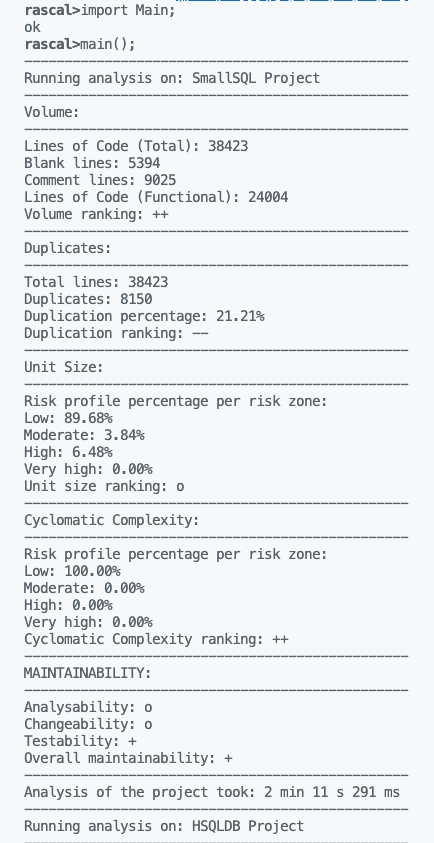
\includegraphics[width=0.7\textwidth]{images/small_sql.png}
    \caption{Terminal result for Small SQL Project}
    \label{fig:small-sql}
\end{figure}

\begin{figure}[h!]
    \centering
    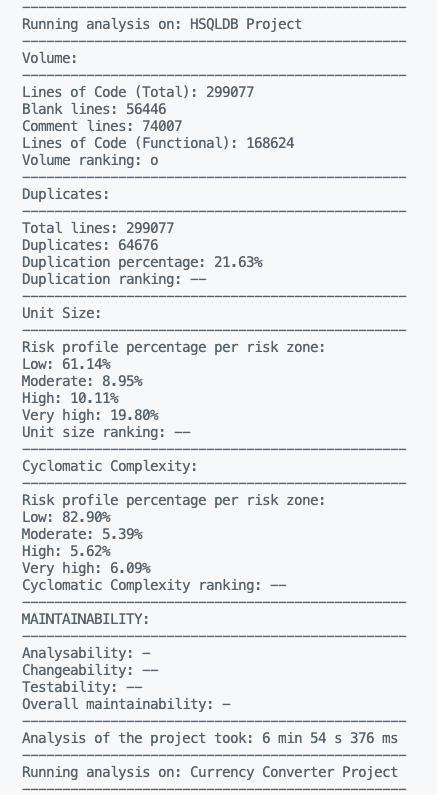
\includegraphics[width=0.7\textwidth]{images/big_sql.png}
    \caption{Terminal result for HSQLDB Project}
    \label{fig:big-sql}
\end{figure}

\begin{figure}[h!]
    \centering
    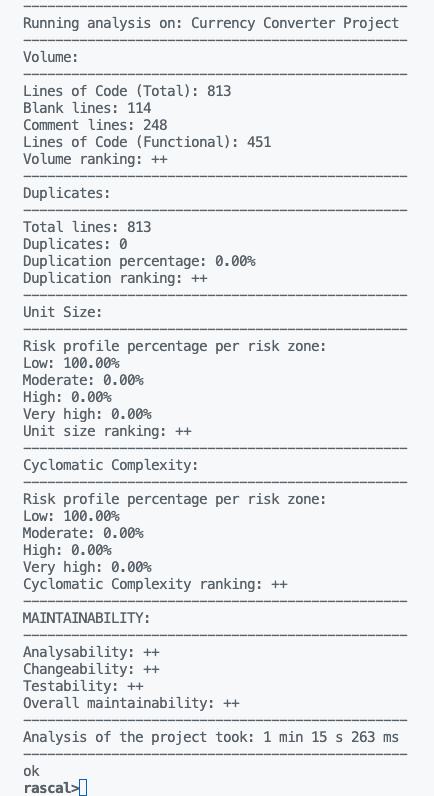
\includegraphics[width=0.7\textwidth]{images/currency_converter.png}
    \caption{Terminal result for Currency Converter Project}
    \label{fig:currency-converter}
\end{figure}

\end{appendices}

\end{document}
